\documentclass[10pt]{article}

%%% Doc layout
\usepackage{fullpage} 
\usepackage{booktabs}       % professional-quality tables
\usepackage{graphicx}       % figure graphics
\usepackage{microtype}      % microtypography
\usepackage{parskip}
\usepackage{times}


%% Hyperlinks always black, no weird boxes
\usepackage[hyphens]{url}
\usepackage[colorlinks=true,allcolors=black,pdfborder={0 0 0}]{hyperref}

%%% Math typesetting
\usepackage{amsmath,amssymb}
\usepackage{pythonhighlight} 

%%% Write out problem statements in purple, solutions in black
\usepackage{xcolor}
\newcommand{\officialdirections}[1]{{\color{purple} #1}}

%%% Avoid automatic section numbers (we'll provide our own)
\setcounter{secnumdepth}{0}

%% --------------
%% Header
%% --------------
\usepackage{fancyhdr}
\setlength{\headheight}{12.0pt}
\fancyhf{}
\fancyhead[C]{\ifnum\value{page}=1 CS 152 L3D - 2024f - HW1: Transfer Learning \else \fi}
\fancyfoot[C]{\thepage} % page number
\renewcommand\headrulewidth{0pt}
\pagestyle{fancy}


%% --------------
%% Begin Document
%% --------------
\begin{document}

~~\\ %% add vertical space

{\Large{\bf HW1: Tung Pham }}

\Large{\bf Collaboration Statement:} This assignment was completed with
collaboration on concept discussion, code-debugging and idea exchange from Arman
Muratbayev, Avtar Rekhi and Joseph Hadidjojo

Total hours of human time: approx. 10-15 hours

Total hours of machine time: approx. 10-15 hrs


~~\\
~~\\
Links: 
\href{https://www.cs.tufts.edu/cs/152L3D/2024f/hw1.html}{[HW1 instructions]} 
\href{https://www.cs.tufts.edu/cs/152L3D/2024f/index.html#collaboration}{[Course collaboration policy]} 

\setcounter{tocdepth}{2}
\tableofcontents

\newpage

\subsection{1a: Figure}
\renewcommand{\figurename}{Fig.}
\renewcommand{\thefigure}{1a}
 \begin{figure}[!h]
     \centering
     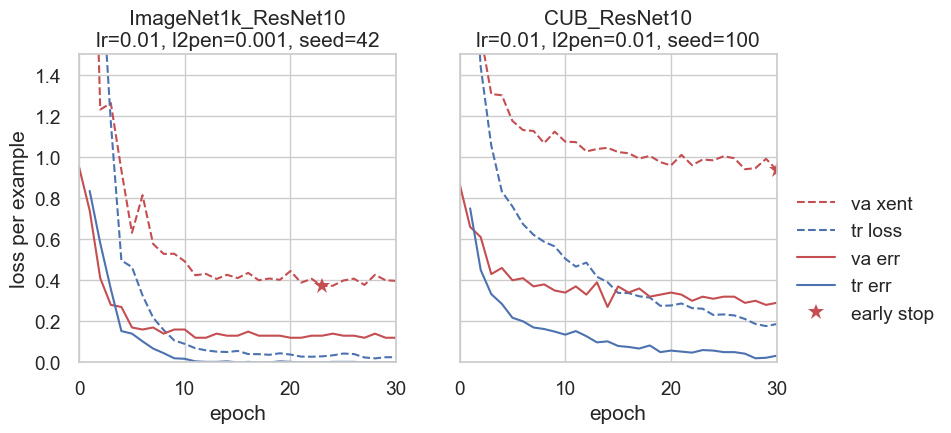
\includegraphics[height=.4\textwidth]{./Figure 1A.png}
     \label{fig:1a}
\caption{
  The two graphs display the curve trends of the losses and error of two
  different models that was trained on 2 different dataset. They all converge
  nicely and there is no sign of overfitting as there isn't any upward trends in
  the validation loss or error while there is a downwards trends or decrease in
  the training loss or error which indicates that both models are fitting the
  training set very well. The model that was trained on ImageNet1k decrease
  rathar quicker than CUB and flattens out and not improving until
  early-stopping occurs. However, we can see that the
  validation cross-entropy value is converging at a rather higher value compares
  to error which indicates that the model is not very confident in its
  selection. As for model that was trained on CUB dataset, the training loss is
  rather slower to converge as we can still see sign of decreasing after we've
  finished the whole epochs. However, for the losses and validation
  cross-entropy value is comparatively fast to converge to the model trained ImageNet1k
  dataset. There is also a sign of unconfidence detected in this model as well
  since we're seeing a significant larger value of cross-entropy compares to the
  training loss at each epoch for this model. In conclusion, it seems that the
  model trained with ImageNet1k generalize better than the model that trained
  with CUB as the validation loss and training loss are closer to each other.
  During experimenting, early stopping helps boost the training process
  significantly as it reduce the need for further computation on some instance
  which reduce the time to conduct grid search on the hyperparameters. I've
  test with multiple a stronger L2 penalty but the effect on the loss value
  seems unnoticeable.
}%endcaption
 \end{figure}

\newpage

\subsection{1b: Figure}
\renewcommand{\figurename}{Fig.}
\renewcommand{\thefigure}{1b}
 \begin{figure}[!h]
     \centering
     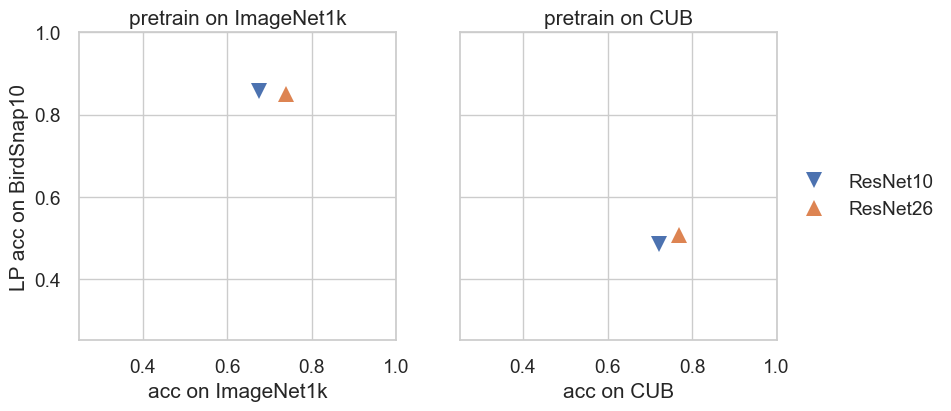
\includegraphics[height=.4\textwidth]{./Figure 1B.png}
     \label{fig:1b}
\caption{
  From the plot, we can see that the model pretrained on the ImageNet1k perform
  better than pretrained on CUB. We can also see that the result obtained from
  our model exceed the top-1 accuracy on Pytorchcv model using ResNet10 on
  ImageNet1k dataset. This confirms the observation of Fang et. al. in his "Does
  progress on ImageNet transfer to real-world datasets" as we can see that this
  models perform exceedingly well on the ImageNet dataset, however, when
  transferring to another dataset like CUB, the performance of the model
  significantly drop. Another note is that on both of our graph, using a larger
  model indeed improve the accuracy which confirms that a larger model with more
  layers and capacity indeed improve our performance which support Fang's claim
  that the model complexity can help in transfer tasks in some cases.
}%endcaption
 \end{figure}

\newpage 


\subsection{2a: Solution}
\renewcommand{\thefigure}{2a}
 \begin{figure}[!h]
     \centering
     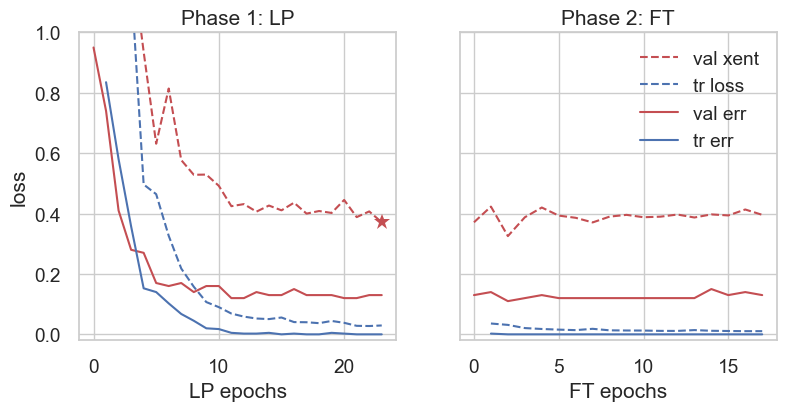
\includegraphics[height=.4\textwidth]{./Figure 2A.png}
     \label{fig:2a}
\caption{
  In this experiment, a grid search was conducted to find the best
  hyperparameters for the fine-tuning phase. However, because we're keeping the
  hyperparameters from previous experiements which fits the data too well, we can see little to no
  gain on the second phase of the training. In the first phase, we can see the
  clear sign of improvements gained from the Linear Probing where the loss and
  error rates drop quickly into convergence around epoch 10. However, in the
  second phase, as we've hope that the Fine tuning on the last 3 layers would
  help further reduce the loss and error rate down, we didn't see this result
  from the graph. In the second phase, the losses and error remains constants
  through out the training with minimal to no drop on any benchmarks. It almost
  have an upward trend which is an indication of overfitting of the second
  model. It could potentially because in the first phase, the model has fit too
  well on the data cause limited to no room in improving the scores on the
  second phase and potentially causing overfitting. This indicates a failure in our implementation to achieve the improvement of this
  approach.
}%endcaption
 \end{figure}

\subsection{2b: Solution}

\begin{verbatim}
    method      test acc
    ------      --------
    LP          0.857
    LP-then-FT  0.850
\end{verbatim}

Here we can see that LP-then-FT is actually not improving our test accuracy but
instead made it worsen. This is due to the fact that it was not improving the
loss or errors rate during training and potentially cause overfitting as we kept
on training. This could be because during Linear Probing, the model has already
fit too well on the dataset which cause limited space for improvements during
Fine Tuning and potentially cause overfitting on this phase. As seen in the
graph before, the graph have an almost upward trend which potentially is the
sign of overfitting and cause of this degration in accuracy on unseen data.

\newpage

\subsection{3a: Concept Question}

Given that $z_i$ represent the logits vector for example i, we can say the
following:
\[
  L_{z_i = x_i + b}
\]

where b is the vector of bias parameters of last layer and $x_i$ is the input
vector which is assumed to have the size of 64x3x244x244. This means that $x_i$
is an input of 64 images and each image has 3 channel. The size of each image is
244x244 which makes i is in the range of 1 to 64.

For simplicity, let's assume that there is no activate function being used here
for forward propagation.
Since in our model predict\_proba we call softmax on the forward, we can come up with the
following formula for softmax:

\[
  {-\log\left( \frac{\exp(z_{i, y_i})}{\sum_{c=1}^{C} \exp(z_{i, c})} \right)}
\]

Our L2 penalty can be written as the sum of square of all the weights which is
defined as follow:

\[
\lambda \sum_{j=1}^{d} \sum_{c=1}^{C} w_{c,j}^2
\]

Where $\lambda$ is the L2 penalty magnitude, C is the number of classes for
classification which is 10 and weight w which has the size d by C where d is the
dimension of the previous layer AveragePool2D of 512 and C is 10.

To finalize our loss function, we just need to take the L2 penalty and add to the normalized softmax
across the batch which give us the following:
\[
L_{\text{total}} = \frac{1}{B} \sum_{i=1}^{B} -\log\left( \frac{\exp(z_{i, y_i})}{\sum_{c=1}^{C} \exp(z_{i, c})} \right) + \lambda \sum_{j=1}^{d} \sum_{c=1}^{C} w_{c,j}^2
\]

\end{document}

